\section{Key Derivation}
\label{appendix:keyderivation}

During a protocol execution, a node derives a master secret $s_i$ from the SPHINX header that is then used to derive multiple sub-secrets for multiple purposes by using the BLAKE2s hash function within HKDF. HKDF is given by two algorithms: $\mathsf{extract}$ and $\mathsf{expand}$, where $\mathsf{extract}$ is used to extract the entropy from a given secret $s$, such as an elliptic-curve point, and produces the intermediate keying material (IKM). The IKM then serves as a master secret to feed $\mathsf{expand}$ in order to derive pseudorandom subkeys in the desired length.

\subsection{Extraction}

As a result of the packet creation and its transformation, the sender is able to derive a shared secret $s_i$ given as a compressed elliptic-curve point (33 bytes) with each of the nodes along the path.

$$s_i^{master} \longleftarrow \mathsf{extract}(s_i, 33, pubKey)$$

By adding their own public key $pubKey$ as a salt, each node derives a unique $s_i^{master}$ for each $s_i$.

\subsection{Expansion}

Each subkey $s_i^{sub}$ is used for one purpose, such as keying the \textit{pseudorandomness generator} (PRG).

$$s_i^{sub} \longleftarrow \mathsf{expand}(s_i^{master}, length(purpose), hashKey(purpose))$$

\begin{center}
    \begin{tabular}{|c | c| c | l |}
        \hline
        Usage                           & Purpose         & Length   & Hash Key (UTF-8)                \\
        \hline
        \hline
        \multirow{3}{*}{SPHINX packet}  & PRG             & 32       & \texttt{HASH\_KEY\_PRG}         \\
                                        & PRP             & 128 + 64 & \texttt{HASH\_KEY\_PRP}         \\
                                        & Packet tag      & 32       & \texttt{HASH\_KEY\_PACKET\_TAG} \\
        \hline
        \multirow{2}{*}{Proof of Relay} & acknowledgement & 32*      & \texttt{HASH\_KEY\_ACK\_KEY}    \\
                                        & ownKey          & 32*      & \texttt{HASH\_KEY\_OWN\_KEY}    \\

        \hline
    \end{tabular}
\end{center}

The values marked with a * are treated as field elements, hence there exists a non-zero probability that $\mathsf{expand}$ produces a value outside of the field. In this specific case, the utilized hash key is repeatedly padded by ``\_'' until $\mathsf{expand}$ returns a field element.

\section{LIONESS wide-block cipher scheme}

\begin{figure}[H]
    \centering
    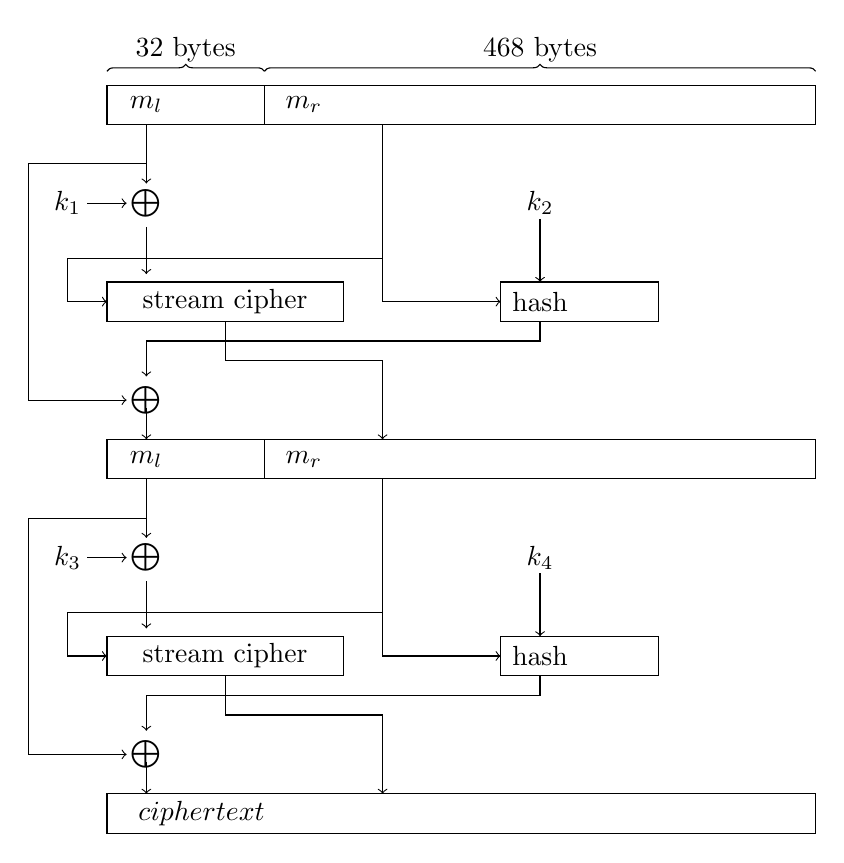
\begin{tikzpicture}
        \def\hashLength{2}
        \def\cipherLength{7}
        \draw[decoration={brace,raise=5pt},decorate] (0,0.5) -- node[above=5pt] {32 bytes} (\hashLength,0.5);
        \draw[decoration={brace,raise=5pt},decorate] (\hashLength,0.5) -- node[above=5pt] {468 bytes} (\hashLength+\cipherLength,0.5);

        \foreach \i\j\offset in{1/2/0,3/4/-4.5} {
                \begin{scope}[shift={(0,\offset)}]
                    \draw (0,0) rectangle (\hashLength,0.5);
                    \draw (\hashLength,0) rectangle (\hashLength+\cipherLength,0.5);

                    \draw (0.5,0.25) node {$m_l$};
                    \draw (\hashLength+0.5,0.25) node {$m_r$};

                    % Encryption
                    \draw (0.5,-1) node {$\bigoplus$};
                    \draw (-0.5,-1) node {$k_\i$};

                    \draw [->] (0.5,0) -- (0.5,-0.75);
                    \draw [->] (-0.25,-1) -- (0.25,-1);
                    \draw [->] (0.5,-1.3) -- (0.5,-1.9);

                    \draw (0,-2.5) rectangle (3, -2);
                    \draw (1.5, -2.25) node [align=center] {stream cipher};

                    % into stream cipher
                    \draw [->] (\hashLength+1.5, 0) -- (\hashLength+1.5, -1.7) -- (-0.5,-1.7) -- (-0.5,-2.25) -- (0,-2.25);

                    \draw [->] (1.5,-2.5) -- (1.5,-3) -- (\hashLength+1.5,-3) -- (\hashLength+1.5,-4);

                    %Hashing
                    \draw (5.5,-1) node {$k_\j$};

                    \draw [->] (5.5,-1.2) -- (5.5,-2);

                    \draw (5,-2.5) rectangle (7, -2);
                    \draw (5.5, -2.25) node [align=center] {hash};

                    \draw [->] (5.5,-2.5) -- (5.5, -2.75) -- (0.5,-2.75) -- (0.5,-3.2);
                    \draw (0.5,-3.5) node {$\bigoplus$};

                    \draw [->] (0.5,-0.5) -- (-1,-0.5) -- (-1,-3.5) -- (0.25,-3.5);
                    \draw [->] (0.5, -3.6) -- (0.5, -4);

                    %m_r into hash
                    \draw [->] (\hashLength+1.5,-1.7) -- (\hashLength+1.5, -2.25) -- (5,-2.25);
                \end{scope}
            }

        \begin{scope}[shift={(0,-9.0)}]
            \draw (0,0) rectangle (\hashLength+\cipherLength,0.5);
            \draw (1.2,0.25) node {$ciphertext$};
        \end{scope}

    \end{tikzpicture}
    \caption{Encryption using LIONESS \cite{lionesspaper} scheme}
\end{figure}

\begin{comment}

\vspace{1cm}
\begin{tabular}{ c | c | c | c | c}
    Name        & Definition & DataType & Size in bytes & usage \\ \hline
    Recipient   &            & address  &               &       \\
    Amount      &            & uint256  &               &       \\
    TicketIndex &            & uint256  &               &       \\
    Iteration   &            & uint256  &               &       \\
    WinProb     &            & uint256  &               &       \\
    Epoch       &            & uint256  &               &       \\
    Challenge   &            & bytes32  &               &       \\
    ChainId     &            & uint8    & 1             &       \\
    Version     &            & uint8    & 1             &       \\
    Tag         &            & uint8    & 1             &       \\
    SignatureX  &            & bytes32  & 32            &       \\
    SignatureY  &            & bytes32  & 32            &
\end{tabular}
\end{comment}